\documentclass[5p,authoryear]{elsarticle}
\makeatletter
\def\ps@pprintTitle{%
 \let\@oddhead\@empty
 \let\@evenhead\@empty
 \let\@evenfoot\@oddfoot} % Supprimer le bas de page ELSEVIER
\makeatother
\usepackage[utf8]{inputenc} % En unicode
\usepackage[T1]{fontenc}
\usepackage[french]{babel}
\usepackage[babel=true]{csquotes} % permet de faire \enquote{a} (« a »)
\usepackage[fleqn]{amsmath} % pour certains signes mathématiques
\usepackage{amsthm} % Pour \begin{gather}
\usepackage{booktabs} % pour \toprule (un style de tableau)
\usepackage{multirow} % Pour colonnes multiples des tableaux
\usepackage{amssymb} % Pour \leqslant (<=, >=)
\usepackage{float}
\usepackage{hyperref} % DOIT ETRE EN DERNIER
\usepackage[french]{cleveref}
\usepackage{graphicx}
\usepackage[margin=0.5in,showframe]{geometry}
\setlength{\parindent}{0pt}
%%------------------------------
\usepackage{tcolorbox}
\tcbuselibrary{skins}
\bibliographystyle{elsarticle-harv}

\begin{document}

\begin{frontmatter}

\title{\textbf{Metropolis algorithm for Ising model and Domain wall dynamics simulation}}

\author{Sagar Prakash Barad$^1$, 2011137}
\address{$^1$School of Physical Sciences, National Institute of Science Education and Research, HBNI, Jatni-752050, India}


\begin{abstract}
  The goal of this paper is to study numerically evolving simple models of materials through a set of microstates in order to determine the thermodynamic averages of measurable quantities.
  We have used monte carlo Metropolis algorithm to study evolution of a microstate q or any therodyanmic quantity A(q) using 2D Ising model. The second part of the paper briefly touches on simulation the Coarsening phenomenon in material using the said model. The end results provides insights for the above physical systems that is complementary to both experiment and theory.
\end{abstract}
\end{frontmatter}

%\linenumbers
\section{Motivation}
For an effective simulation we need an algorithm that could efficiently and more importantly accurately calculate the equilibrium thermodynamic averages of model systems. MC simulation
generate a sequence of states chosen by a random walk among the configurational microstates of the canonical ensemble.Then takes takes the ensemble average for all available states and then by the \textbf{law of large numbers (LLN)}, theoretically the results should be close to the  and tends to become closer to the expected value as more trials are performed. Metropolis algorithm is subsection of MC importance sampling, which greatest strength is that most of the computational power is spent on generating microstates that are representative of the equilibrium
ensemble rather than sampling all of the phase space. It is this huge improvement in efficiency that makes computer simulations of statistical mechanical models feasible.

\section{Theory}
\begin{figure}[h]
  \centering
  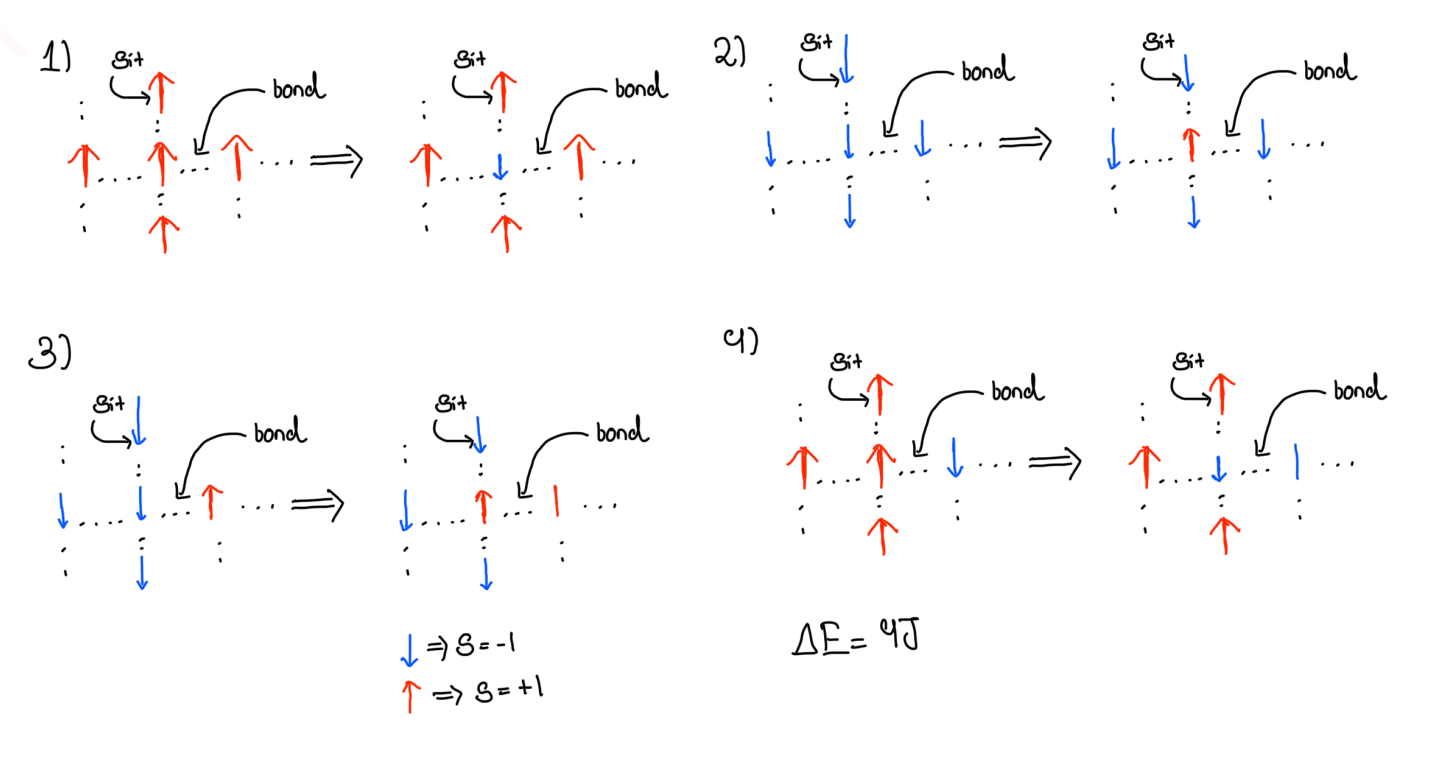
\includegraphics[width=0.4\textwidth]{2.png}
  \caption{Here $S = 1$ and $S = -1$ are used for up and down configuration of the spins. And all the transitions mentioned in the above figure is $\Delta E = 4J$.}
\end{figure}
\subsection{Ising model}
An Ising model is a mathematical model of ferromagnetism (for example, iron can be magnetized in a magnetic field, but if heated, it loses magnetization beyond Curie temperature). Named after Ernst Ising, Ph.D. in Physics (1924) from the University of Hamburg under the supervision of Wilhelm Lenz. Ising solved the one-dimensional (1D) Ising model exactly to find no phase transition. He also provided arguments on why there would not be a phase transition in higher dimensions either. In 1936, Peierls argued that both 2D and 3D Ising models admit phase transitions. The argument is summarised below.

The Ising Hamiltonian can be written as,

$$\mathcal{H} = -J \sum_{\langle i j \rangle} S_{i} S_{j} - H\sum_{\langle i \rangle} S_{i}.$$

\begin{enumerate}
  \item The spins $S_i$ can take $\pm 1$.
  \item Main idea behind the Ising model is it restriction interactions to nearest neighbour $\langle ij \rangle$ only.
  \item $J > 0$ coefficient is indicative of strength of exchange interaction.
  \item $H$ is the applied magnetic field.
\end{enumerate}

The system undergoes a second order phase transition at the critical temperature $T_{c}$. For temperatures less than $T_{c}$, the system magnetizes, and the state is called the ferromagnetic or the ordered state. This amounts to a globally ordered state due to the presence of local interactions between the spin. For temperatures greater than $T_{c}$, the system is in the disordered or the paramagnetic state. In this case, there are no long-range correlations between the spins.

The order parameter

$$m = \frac{1}{N}\sum_i S_i$$

for this system is the average magnetization. The order parameter distinguishes the two phases realized by the systems. It is zero in the disordered state, while non-zero in the ordered, ferromagnetic, state.

\subsection{Montecarlo Simulations}
A Monte Carlo simulation uses pseudorandom numbers to draw a representative sample of microstates $[q]$ from the equilibrium probability distribution,

\begin{equation}
  P_{eq}(q) = \frac{exp(-\beta E(q)}{\sum_{q'} exp(-\beta E(q')}
\end{equation}

So we choose a configuration with a probability exp(-E/KT) and weight them evenly (Metropolis et al., 1953). Consider an ensemble of microstates that has some initial distribution of probabilities $P(q,0)$ and let the distribution evolve according to the discrete stochastic rate equation\footnote{Algorithm described is originally from Metropolis et al., 1953; Kalos and Whitlock, 1986; Allen and Tildesley, 1990; Frenkel and Smit, 2002; Binder and Heermann, 2002; Landau and Binder, 2009}

\begin{equation}
  \Delta P(q,t) = \sum_{q'}P(q',t)W(q' \rightarrow q) - P(q,t)\sum_{q'}W(q \rightarrow q')
\end{equation}

where $W(q \rightarrow q')$ is the transition rate from state $q$ to state $q'$ and $\Delta P(q,t) = P(q,t+1) - P(q,t)$. If the transition rate obeys the balance condition

\begin{equation}
  \sum_{q'}P_{eq}(q')W(q' \rightarrow q) = \sum_{q'}P_{eq}(q)W(q \rightarrow q')
\end{equation}

and the random process in equation (2) can reach every microstate from every other microstate in a finite number of steps, then the ensemble probability will approach the equilibrium distribution:

\begin{equation}
  lim_{t \rightarrow \inf} P(q,t) = Peq(q)
\end{equation}

In practice, equation (3) is usually implemented using the detailed balance condition

\begin{equation}
  P_{eq}(q')W(q' \rightarrow q) = P_{eq}(q)W(q \rightarrow q')
\end{equation}

Evaluating $P_{eq}(q)$ requires summing over all states to determine the partition function, but the ratio $P_{eq}(q')/P_{eq}(q)$ depends only on the energy difference $\Delta E = E(q') \ - \ E(q)$.

Therefore, the transition rates are related by

\begin{equation}
  W(q \rightarrow q') = exp(-\beta \Delta E)W(q' \rightarrow q)
\end{equation}

This guarantees that the sequence of states generated by this stochastic process, beginning from any starting configuration, asymptotically becomes equivalent to selecting states by a random walk among the microstates of the equilibrium ensemble.

\\
Basically,
\begin{equation}
  W(q \rightarrow q') = 1 \ \ if \Delta E \le 0
\end{equation}

\begin{equation}
  W(q \rightarrow q') = exp(-\beta \Delta E) \ \ if \Delta E \ge 0
\end{equation}

\subsection{A Metropolis Monte Carlo algorithm: Psuedocode}
The Metropolis method can be implemented using PRNG (class buitlt LCGPRNG()) that returns pseudorandom numbers that are uniformly distributed on the open unit interval (0.0,1.0).

\begin{tcolorbox}[width=4in,
                  %%enhanced,
                  %%frame hidden,
                  interior hidden,
                  boxsep=0pt,
                  left=0pt,
                  right=0pt,
                  top=2pt,
                  ]%%
  \textbf{Psuedocode}
  \begin{enumerate}
    \item Prepare an initial configuration of N spins.
    \item Flip the spin of a randomly chosen lattice site.
    \item Calculate the change in energy dE.
    \item If $dE < 0$, accept the move. Otherwise accept the move with probability $exp(-dE/T)$. This   satisfies the detailed balance condition, ensuring a final equilibrium state.
    \item Repeat 2-4.
  \end{enumerate}
\end{tcolorbox}

To determine averages at a different set of parameters (temperature, density, etc.), change
the parameters by a small amount and repeat steps 1 through 5, including the equilibration
step 4.5 Using the last configuration of the previous run as the first configuration of the next
run can often reduce the equilibration time.

\begin{figure}[h]
  \centering
  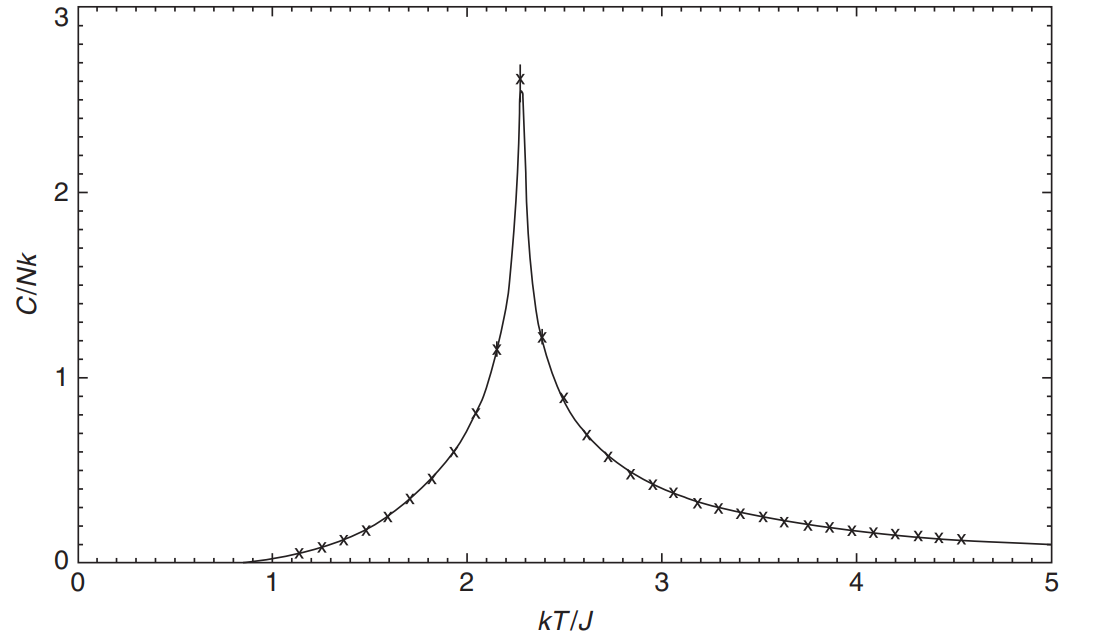
\includegraphics[width=0.4\textwidth]{1.png}
  \caption{Monte Carlo specific heat (×’s) of the two-dimensional Ising model on a 128×128 lattice, as compared to the exact solution (solid line) from Section 13.4.A; see Kaufman (1948), Ferdinand and Fisher (1967), and Beale (1996). The MC error bars are smaller than the symbols used, except near the bulk critical temperature $T_{c}$. Each data point represents an average using $10^5$ Monte Carlo sweeps, except at the bulk critical point where $10^6$ Monte Carlo sweeps were used to mitigate critical slowing down.}
\end{figure}

\section{Results}

\subsection{Phase transitions in 2D Ising model}
 Our code for the Ising model simulation gave us an output for energy, magnetization, specific heat and susceptibility of the system for increasing T.

 \begin{figure}[h]
   \centering
   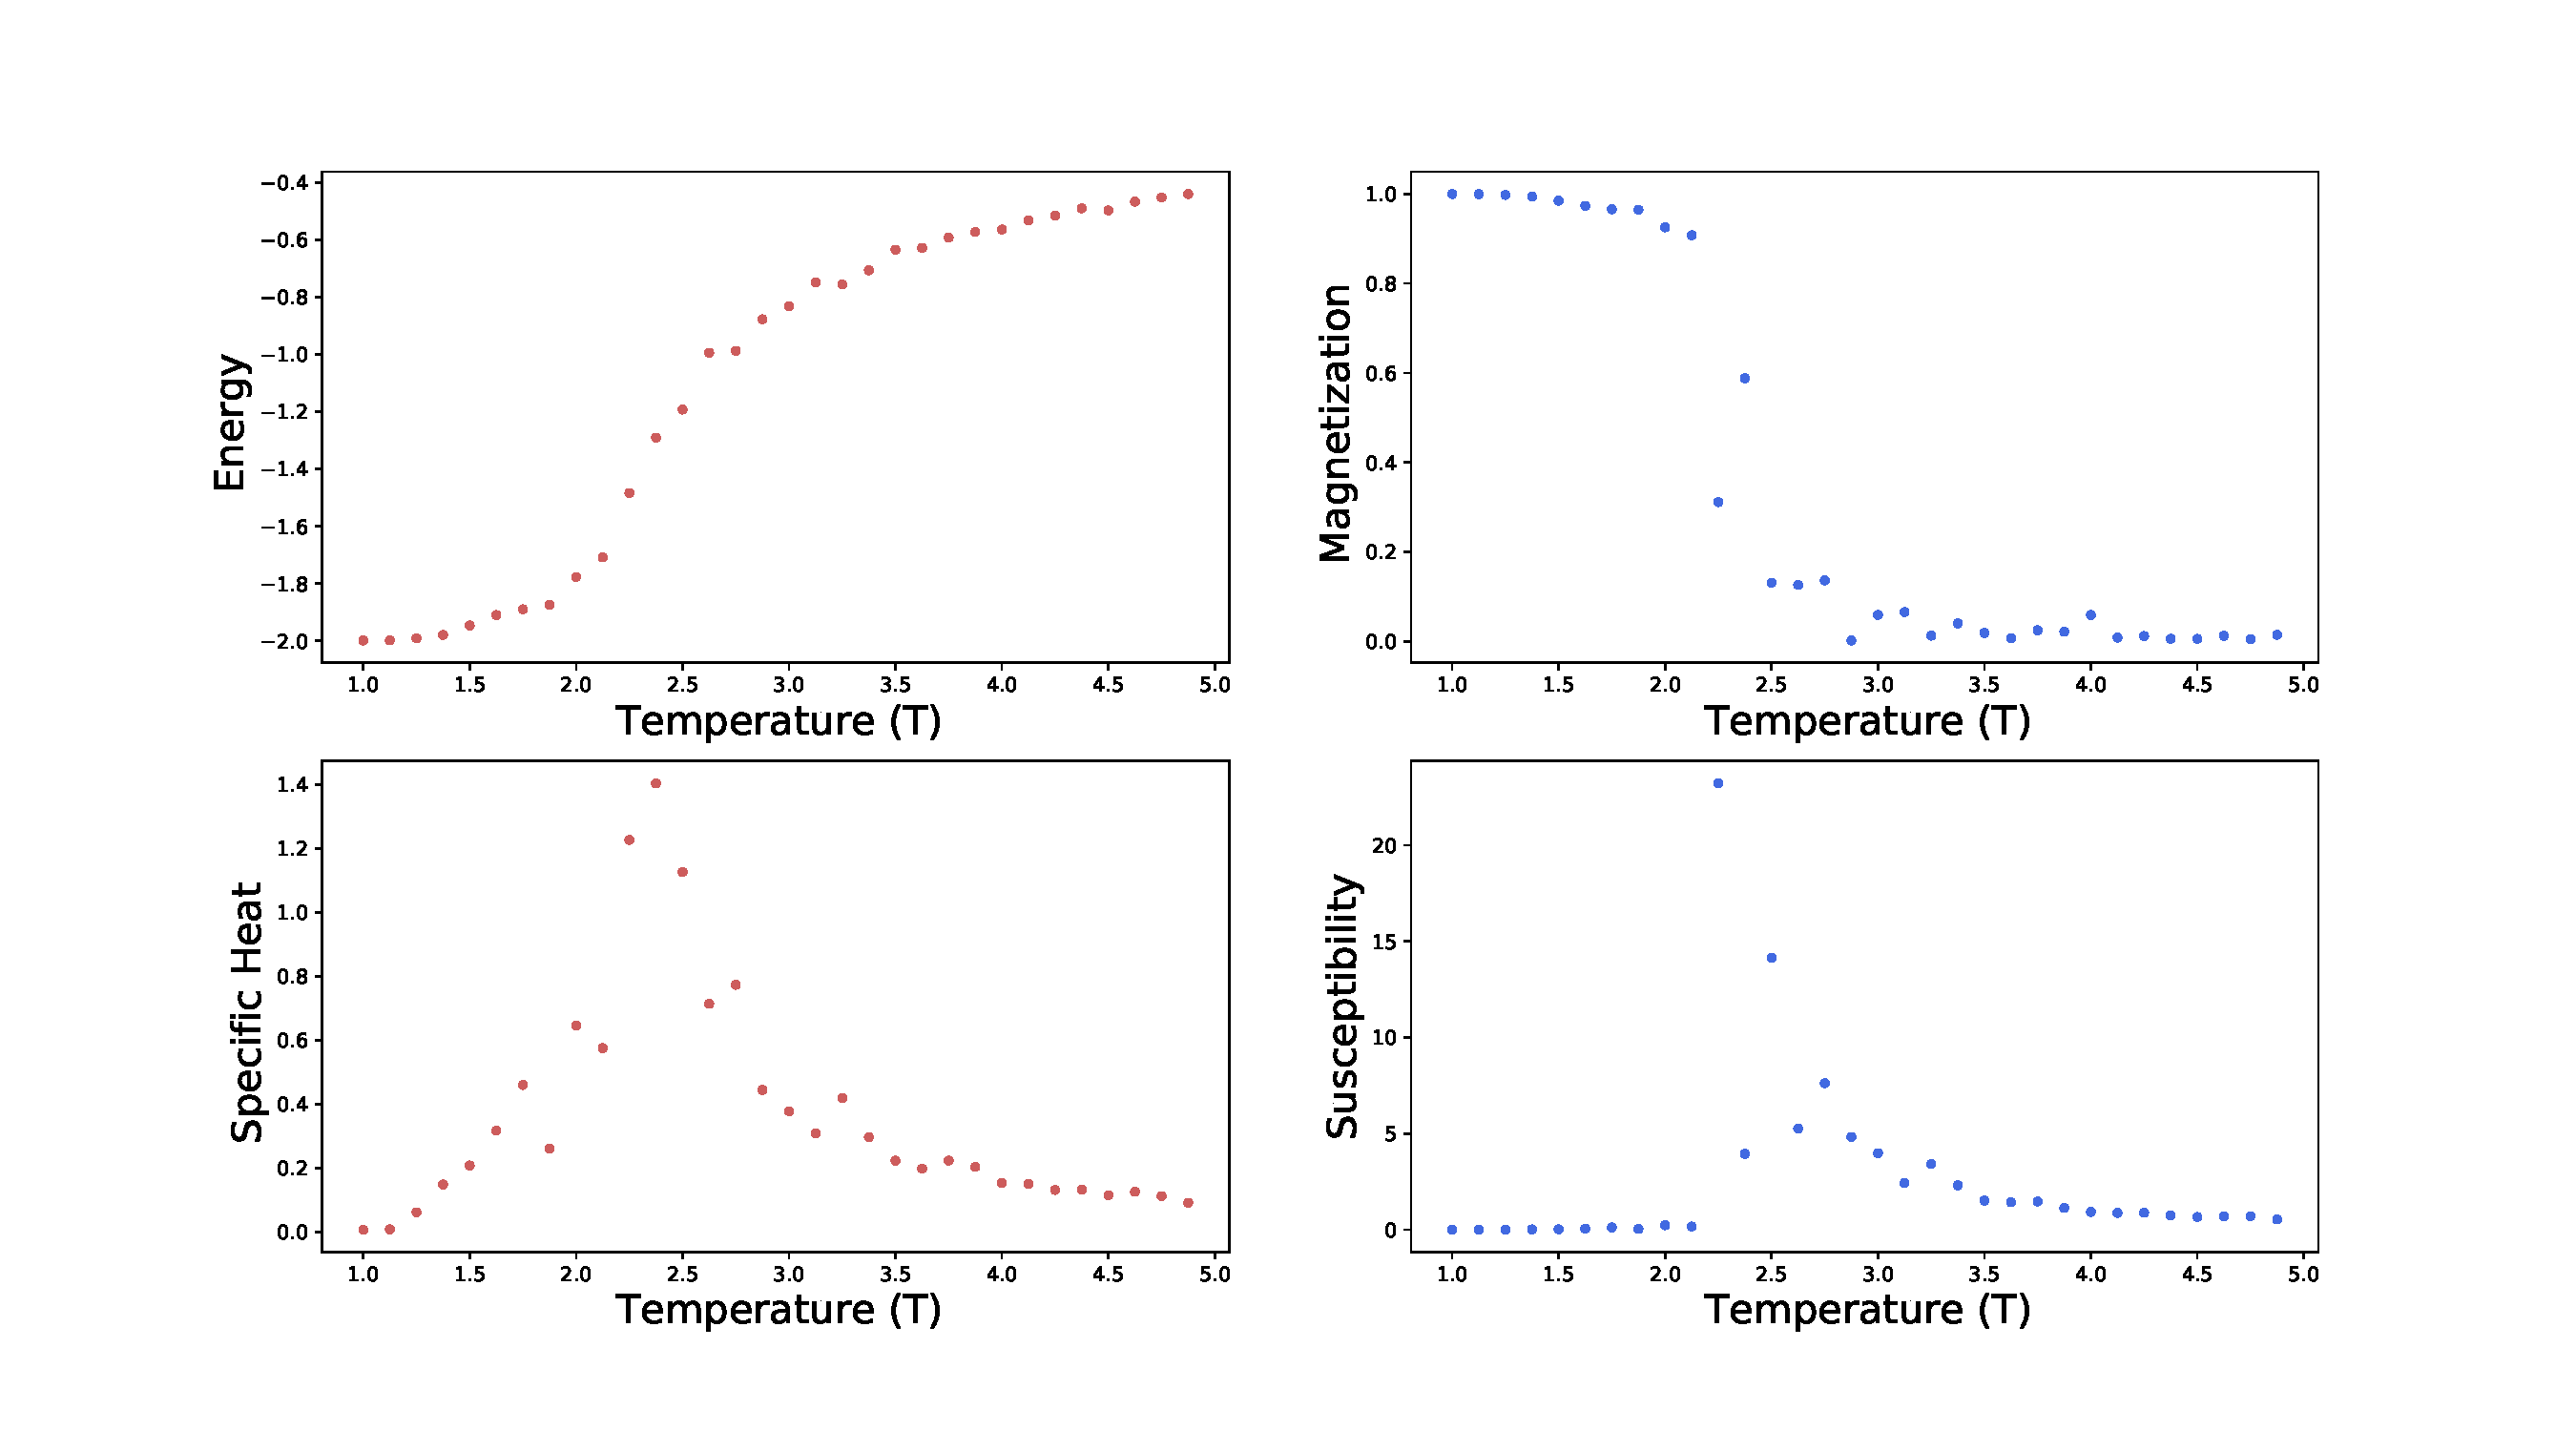
\includegraphics[width=0.5\textwidth]{Phase_transition.pdf}
   \caption{The quantities on the y-axis, in the above plots, are per spin. These intensive quantities have been plotted against temperature on the x-axis. It can be seen that the critical temperature for the numerical simulation of this small system is close to the known value of $T_c \sim 2.269$ for a thermodynamic system.}
 \end{figure}

\subsection{Domain growth in 2D Ising model}
We start with a random initial condition and then plot the instantaneous configurations, as the system  coarsens to its equilibrium state.

\begin{figure}[h]
  \centering
  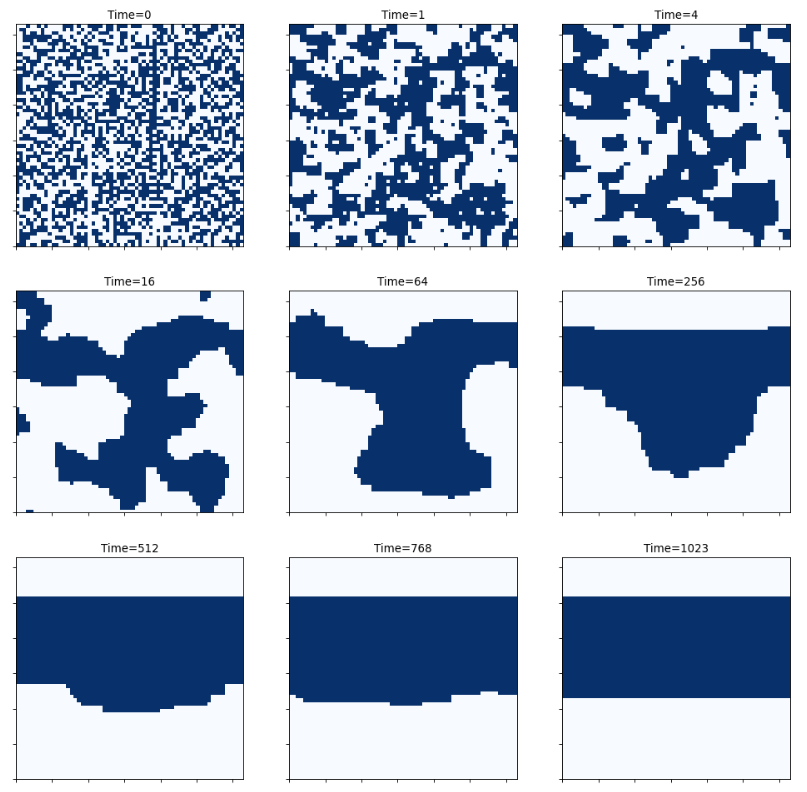
\includegraphics[width=0.4\textwidth]{Domain_growth.png}
  \caption{Time evolution in the spin configuration.The simulation starts from t = 0 with a random spin state and then evolution of state at various time, as the system coarsening to its equilibrium state i.e. Domain wall formation.}
\end{figure}

\section{Caveat with the algorithm}
\begin{enumerate}
  \item Monte Carlo simulations are hampered beacuse the simulation must run long enough for the model to explore a sufficiently large region of the phase space to capture the equilibrium behavior. This issue can be mitigated by special simulation methods such as coarse graining, cluster update methods, parallel tempering, multicanonical Monte Carlo methods, Monte Carlo renormalization group, and so on.
  \item Interactions between particles are usually highly simplified for computational efficiency and the interaction range is usually cut off. Long-range interactions (Couloub, dipole, van der Waals, etc.) need to be resummed or treated via perturbation theory to try to account for their effects.
  \item MC simulations do not directly measure the number of microstates available to the system, so one cannot directly calculate the entropy or the free energy in the same way as other observables.
  \item All pseudorandom number generators produce some level of correlation in their sequences. Even subtle correlations in pseudorandom number sequences can produce erroneous results in Monte Carlo simulations.
  \item Confirming the validity of MC simulation is essential and this process is rather different from verifying a theoretical calculation. Some code
evaluation and verification procedures include: testing the code initially on small systems with known properties, testing the code whenever possible against models with exact solutions or models that have been widely studied in the literature, examining results as a function of system size and run length, and retesting carefully whenever new interactions or code modules are added.
\end{enumerate}

\section{Conclusion}
This FM $\rightarrow$ PM phase transition and Domain wall formation was simulated using the program for Metropolis Algorithm in python but the for accurate results the simulation require fine tuning of paramters which is rather time taking. One futher improve on this algorithm by defining function that autonomously define the parameters for the simulations. The method described provide a huge improvement than rather normal sampling and thus it is an efficient method.

\section{References}
\begin{enumerate}
  \item Pathria, R. K., and Paul D. Beale. Statistical Mechanics. Academic Press, 2021.
  \item \href{https://files.speakerdeck.com/presentations/1d7f8f8af5714772b1ea4d007009655d/kpt.pdf}{Rajesh Singh, Coarsening phenomenon, IISM}
  \item \href{https://en.wikipedia.org/wiki/Ising_model}{“Ising Model - Wikipedia.” Ising Model - Wikipedia, 21 Apr. 2013, en.wikipedia.org/wiki/Ising model.}
\end{enumerate}
\end{document}
